\subsection{Digital Terrain Model}

Modelling sea-induced flooding requires a digital terrain mode (DTM). A DTM is a digital representation of the elevation of the landscape in relation to a reference. A DTM differs from a digital surface model (DSM) by not including buildings and trees \citep{sdfe_dhm_2020}. A DTM is made using LiDAR aerial scanning technology and is recorded in Denmark over a 5-year period in different sections. In Denmark, the Danish Agency for Climate Data (\textit{formerly} The Danish Agency for Data Supply and Infrastructure) is responsible for establishing the DTM from the LiDAR point cloud \citep{sdfe_dhm_2020}.\\

In this study, the latest updated DTM from 2023 has been used. For Aabenraa, Gedser and Hesnæs, the DTM was last recorded in 2023, while the DTM for Præstø is from 2019. DTM for Denmark is stored as GeoTIFF raster format with a cell size of 0.4$times$0.4 metres (0.16m$^{2}$). The DTM is in a UTM zone 32 north projection and in the ETRS89 coordinate system with a horizontal precision of \pm 15 centimetres. The vertical reference is in the Danish Vertical Reference 90 (DVR90) with a vertical precision of \pm 5 centimetres \citep{sdfe_dhm_2020}.\\
To minimize processing time, the DTM was cut down t a demarcation of each area. The demarcation was based on the surrounding topography and the extent of any urbanised zones. In addition, the DTM has been converted to a digital hydrological terrain model (DHyM) and building outlines have been burned in as impassable regions of the terrain.

\subsubsection{Hydrological Adaptations}
To convert a DTM into a DHyM, two hydrological adaptation layers have been used: Line and horseshoe adaptations. The adaptations are both one-dimensional geometric data objects defined by GeoDanmark as polylines \citep{GeoDanmark_HydroLag}.\\
The line adaptations are defined as a single line object that describes an opening for surface water flow through an obstacle or an obstacle to surface water flow through the terrain \citep{DHMLinje}. Line adaptations are the simplest hydrological adaptation and occur, among other things, as pipes and small streams passing under roads or between fields. An example of a line adaptation of a pipe from a field to the sea is shown in figure \ref{Subfig: Linjetilpasning}.\\

Horseshoe adaptations are defined by \cite{DHM_Hestesko}, as a horseshoe-shaped geometric object that allows or restricts the flow of surface water through an obstacle or the terrain. The width of the horseshoe outlines the size of the obstacle in the landscape that are larger than a small stream or pipe and thus require a more correct representation in the landscape. Horseshoe adaptations are found under larger bridges and tunnels under roads. An example of a horseshoe adaptation from a bicycle tunnel under a road is shown in figure \ref{Subfig: Hesteskotilpasning}.
\begin{figure}[H]
	\begin{subfigure}[b]{0.5\textwidth}
		\centering
		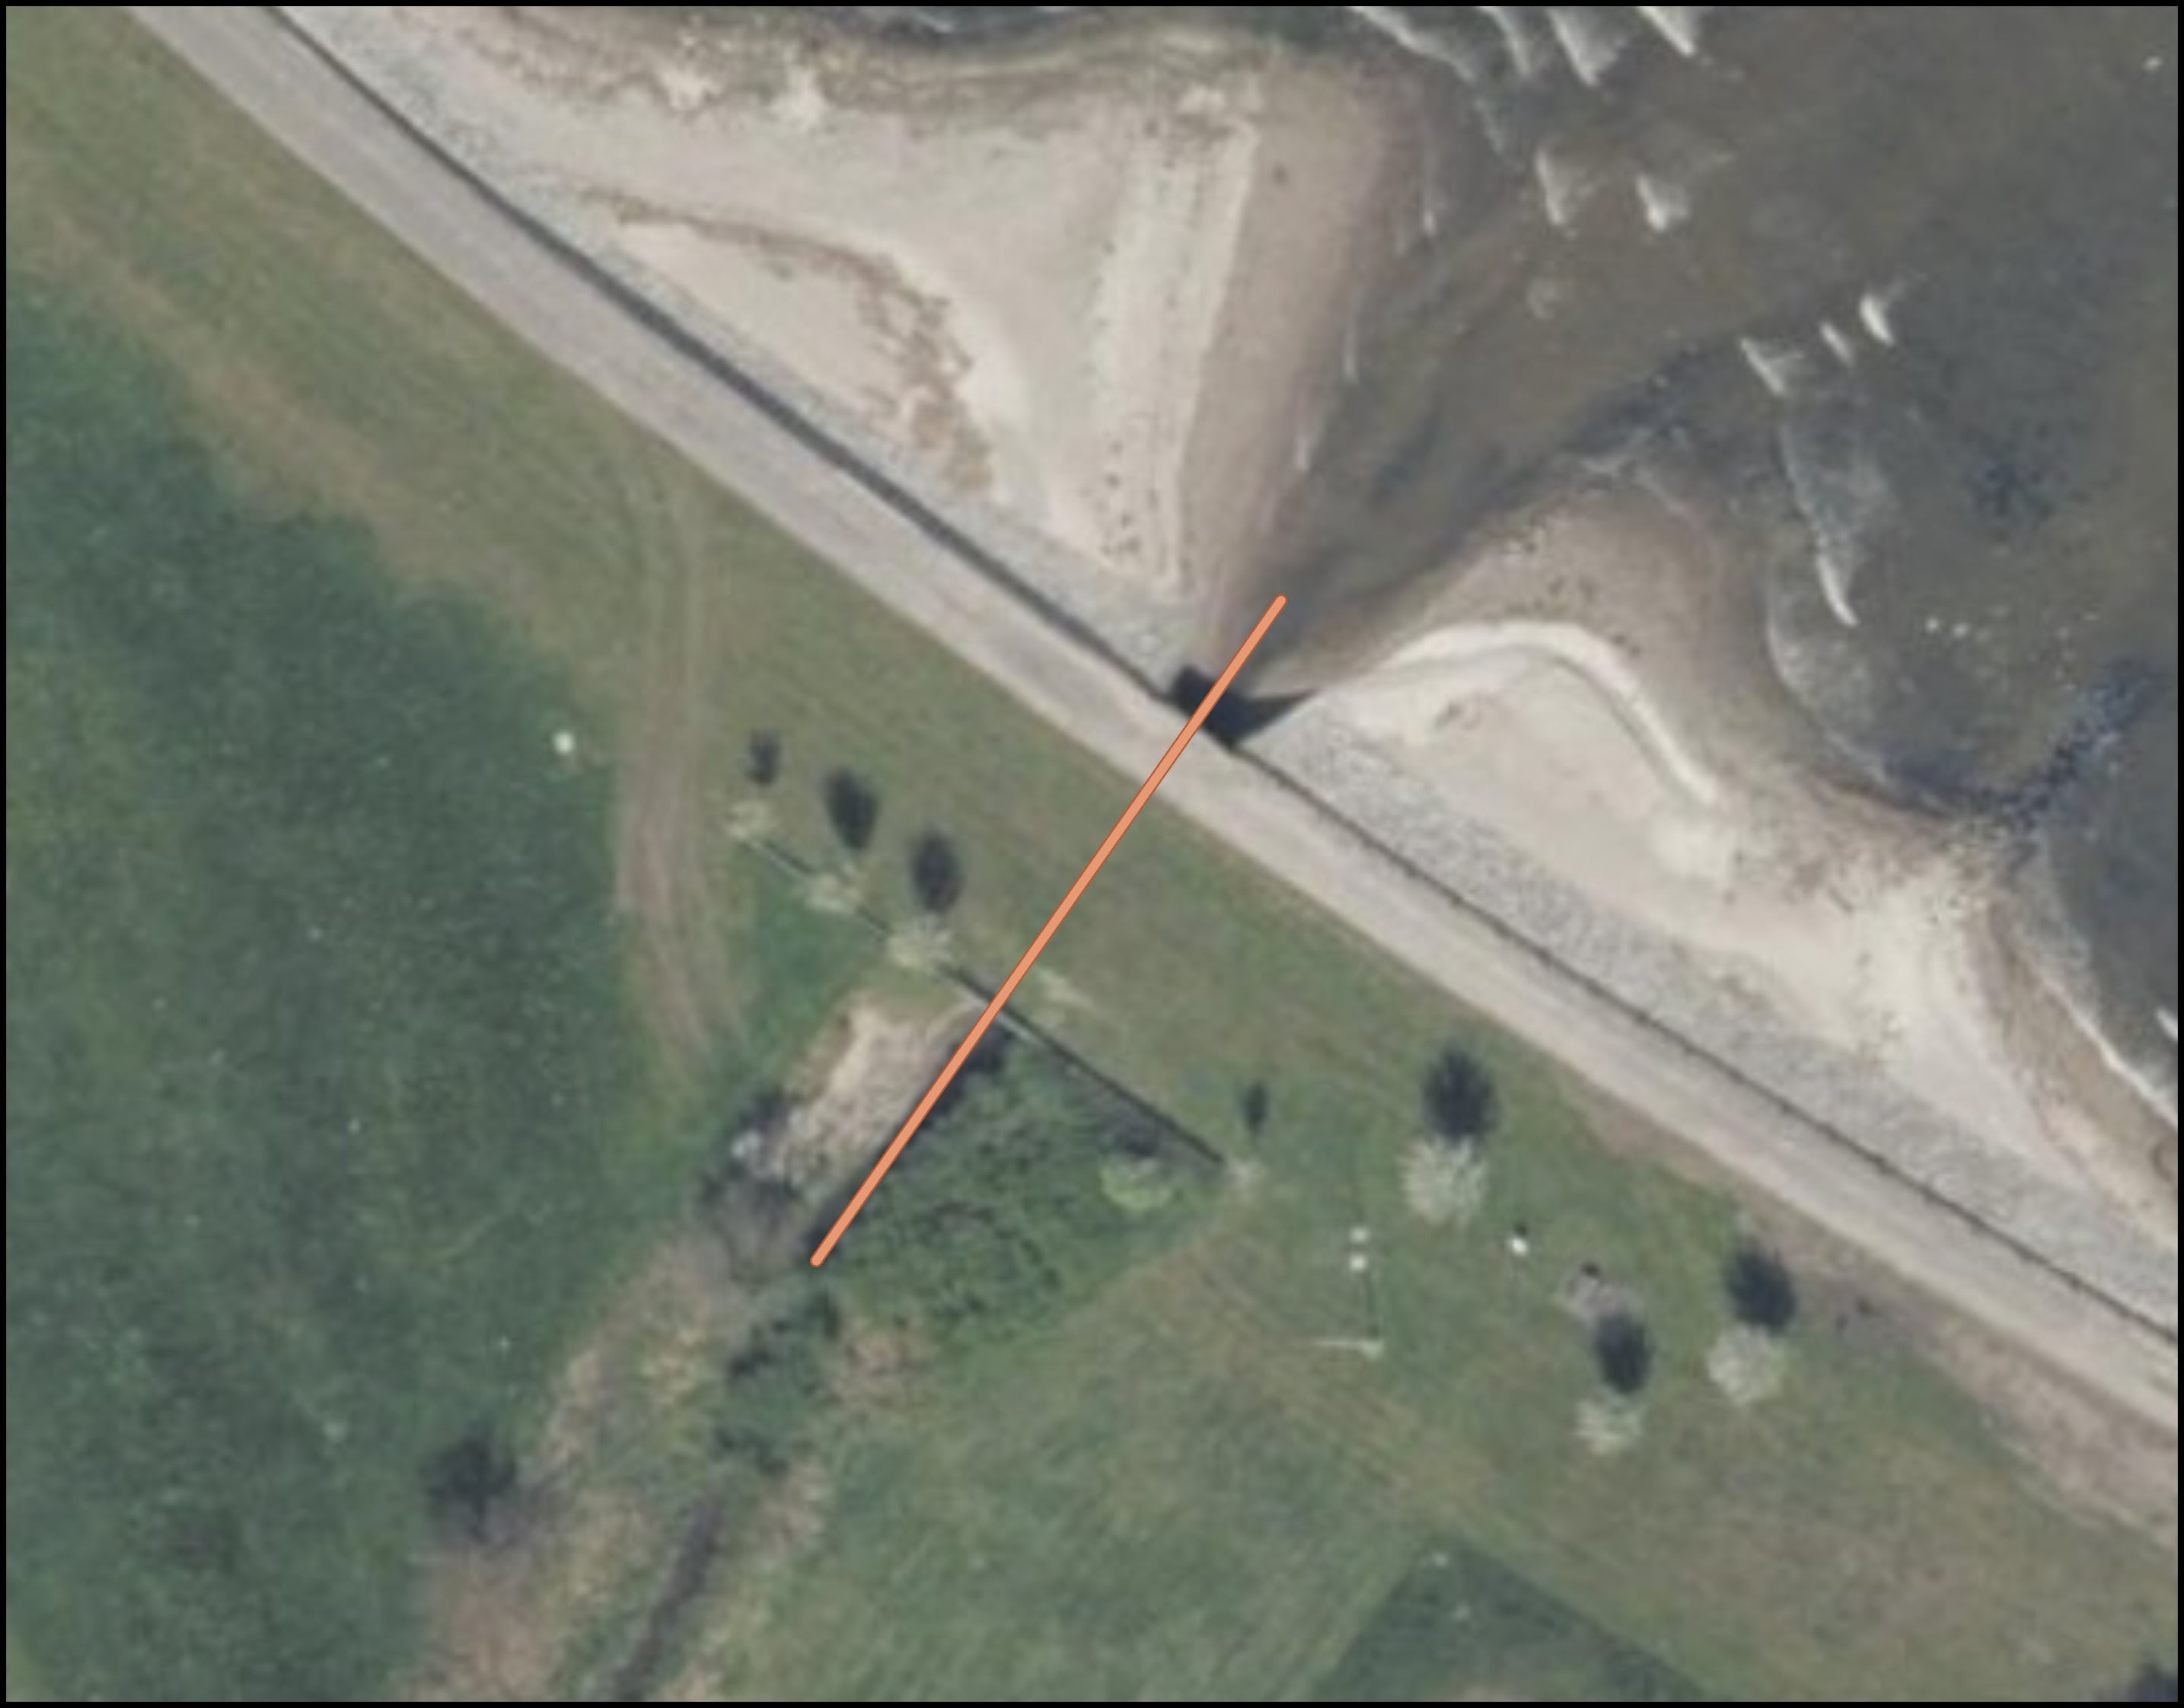
\includegraphics[width=1\linewidth]{images/databeskrivelse/linje.jpg}
		\caption{}
		\label{Subfig: Linjetilpasning}
	\end{subfigure}
	\hspace{0.2cm}
	\begin{subfigure}[b]{0.5\textwidth}
		\centering
		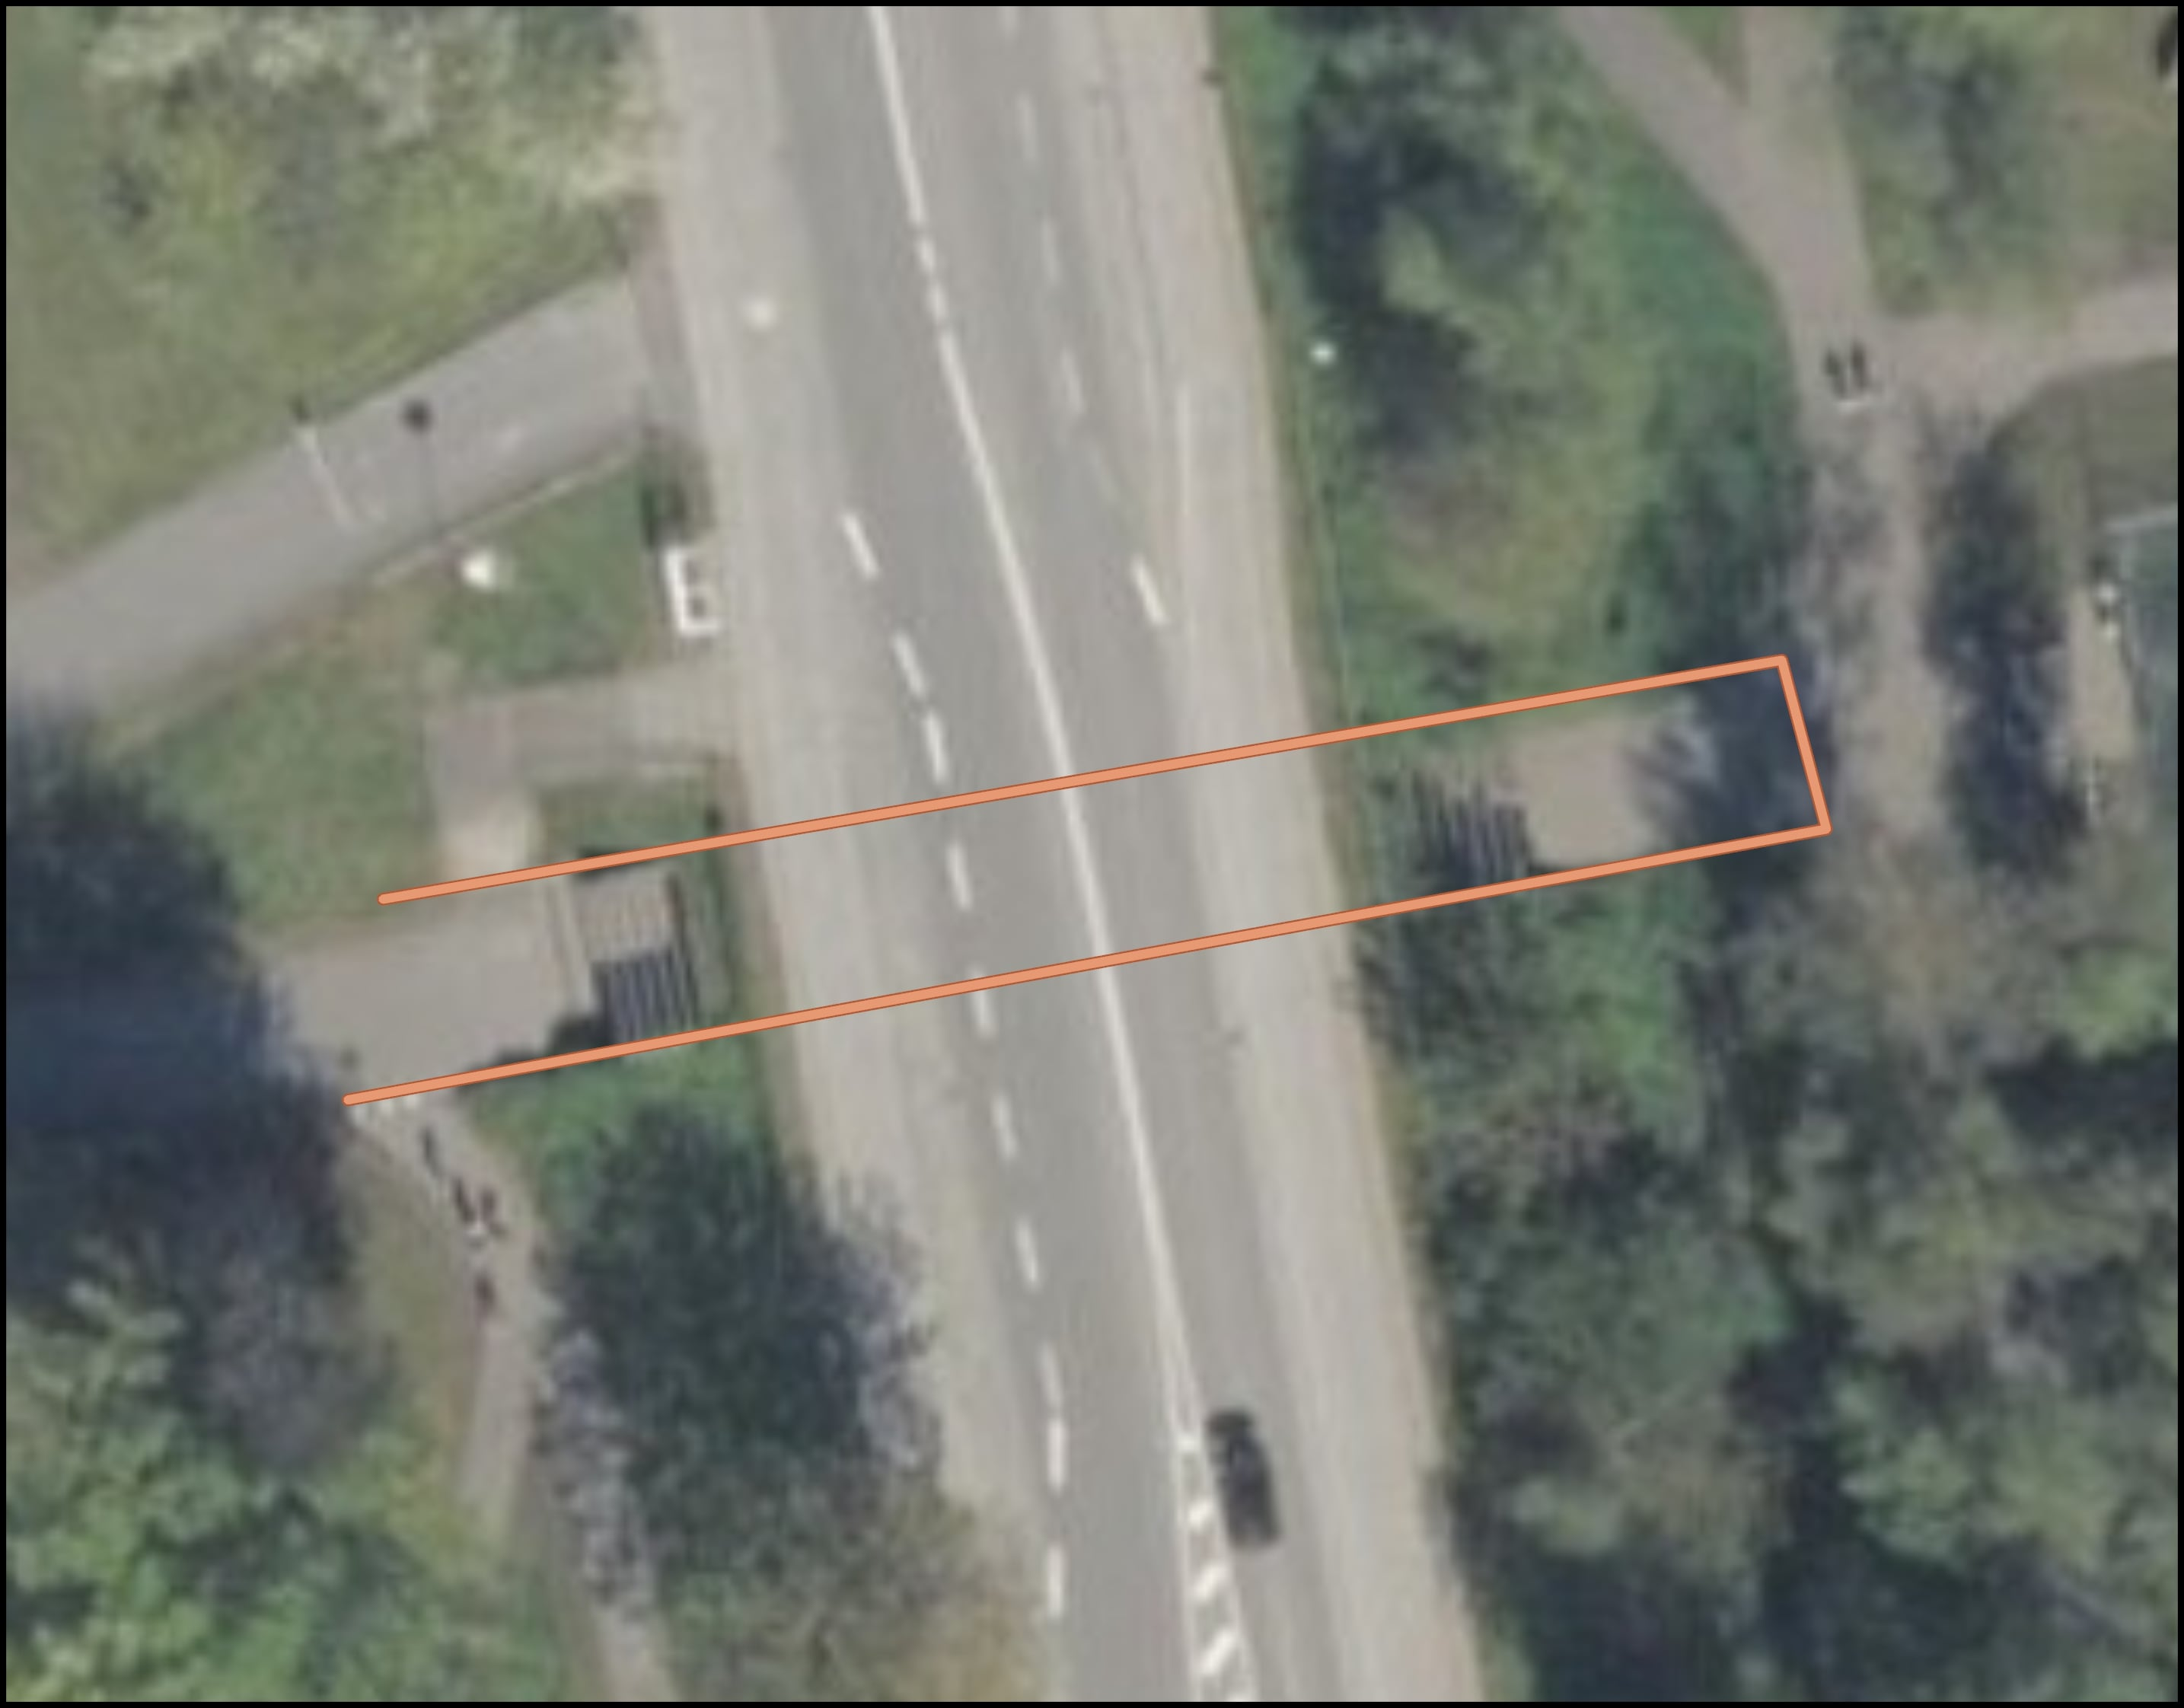
\includegraphics[width=1\linewidth]{images/databeskrivelse/hestesko.jpg}
		\caption{}
		\label{Subfig: Hesteskotilpasning}
	\end{subfigure}
	\caption{Eksempler på en \textbf{(a)} Linjetilpasning fra et mindre vandløb under en græsplæne. \textbf{(b)} Hesteskotilpasning fra en cykeltunnel under en vej i Aabenraa.}
	\label{Figur: Linje- og hesteskotilpasninger}
\end{figure}

\subsubsection{Wind and water level data}
To understand the context behind the storm surge event on 20th-21st of October 2023, wind and water level data for the month of October 2023 have been collected.\\
Wind data has been collected from the Danish Meteorological Institute's (DMI) weather archive \citep{dmi_vejrarkiv} for the entire country and an average, highest 10-min average, and the maximum wind speed in ms$^{-1}$ for each day of the month was calculated.\\

Water level data has been collected in two ways. Data from Gedser, Hesnæs and Præstø have been collected from DMI's Open Data Oceanographic Observation Data API-resource \citep{dmi_open_data}. Water level data is recorded every 10 minutes from October 1st to October 31st 2023 and has been filtered down to a date range from the 15th to 23rd of October. Data for Præstø has been retrieved from Rødvig Havn, approximately 25 km north-east, as Præstø does not have an official DMI water level gauge. This is the same station that \cite{cowi_praesto_2025} used to provide an estimate of the water level measured in Præstø.\\
Water level data from Aabenraa has been collected directly from DMI with permission from the company Aabenraa Harbour, as DMI does not make the port's raw measurements available to the public.\\

The water level data from Gedser Havn had some deviations, where the water level fluctuated from +200 cm to -340 cm in 10 minutes. The data points were removed according to a criterion that the water level could not realistically change by more than \pm 25\% in minutes. If the water level is not within the boundary criteria, the that data point is removed and the following data point is taken into account. If the next data point is within the boundary, then that point becomes the new value that is checked. The logic behind the filtering is shown in equation \ref{Eq: Outlier vandstand}. Where $x$ is a data point in the series and $x_i$ is the following data point in the series.
\begin{align} \label{Eq: Outlier vandstand}
	\text{If } x_i \in [0.75\times x, 1.25\times x], \text{ then } x \leftarrow x_i \nonumber \\
	\text{If } x_i \notin [0.75\times x, 1.25\times x], \text{ then remove } x_i
\end{align}

\subsubsection{Data from study sites and other used data products}
This study used several data received from the three municipalities. The primary data form was a rasterised map of the water spread from the storm surge. All maps were resampled to a cell size of 0.4\times0.4 metres, to ensure the same cell size as the DTM, as all maps had different cell sizes that varied between 0.45 and 0.5 metres.\\
Aabenraa municipality also provided information, line and point data about emergency response efforts, including the locations of placed watertubes and drone images of the city.\\

In addition to the above mentioned data, a number of smaller data products have also been used. This includes a dataset of building polygons from GeoDanmark, which has been used burn the building footprints into the DHyM. A topographic land polygon over Danmark from the Danish Agency for Climate Data has been used as a boundary mask for the Inundation Model's results. A dataset of the sea level rise projections for 2030 from the sixth \cite{ipcc_report_AR6, garner_ipcc_2021} climate report and a tool with station numbers for the projections from \cite{NASA_tool}. This dataset was used to calculate a projected storm surge event in 2100.